%!TEX root = ../thesis.tex

\thispagestyle{myheadings}

\graphicspath{{Body/Figures/TrackingFigures/}{Body/Figures/TrackingFigures/MainPlots/}{Body/Figures/TrackingFigures/MainPlots/PlanePlots/}{Body/Figures/TrackingFigures/MainPlots/PullPlots/}{Body/Figures/TrackingFigures/MainPlots/Residuals/}{Body/Figures/TrackingFigures/eLoss/}{Body/Figures/TrackingFigures/CoordSys/}{Body/Figures/TrackingFigures/TrackerPics/}{Body/Figures/TrackingFigures/Field/}{Body/Figures/TrackingFigures/TrackingFlow/}{Body/Figures/TrackingFigures/LeftRight/}{Body/Figures/TrackingFigures/Misc/}{Body/Figures/TrackingFigures/Extrapolation/}{Body/Figures/TrackingFigures/Tracks/}}

\chapter{Track Reconstruction and Analysis}
\label{chapter:TrackReconstruction}

As was talked about briefly in section \ref{sec:StrawTrackers}, the straw trackers are used to provide information about the muon beam, as well as info for the calorimeters. The straw track reconstruction is performed in several stages. The ``Track Finding'' stage takes incoming hits and decides which hits should be grouped together to form a single track for a single positron. The ``Track Fitting'' stage fits the measured positions of these invidividual hits and forms a single track describing the trajectory of the incident positron. Finally the ``Track Extrapolation'' stage takes the fitted track information and extrapolates the position and momentum components to the regions of interest, namely the storage region and the calorimeter.





-see the previous section for the hardware information...
-Geane (Geometry and Error Propagation)




\section{Track Finding}
\label{sec:TrackFinding}


\begin{figure}[]
	\centering
	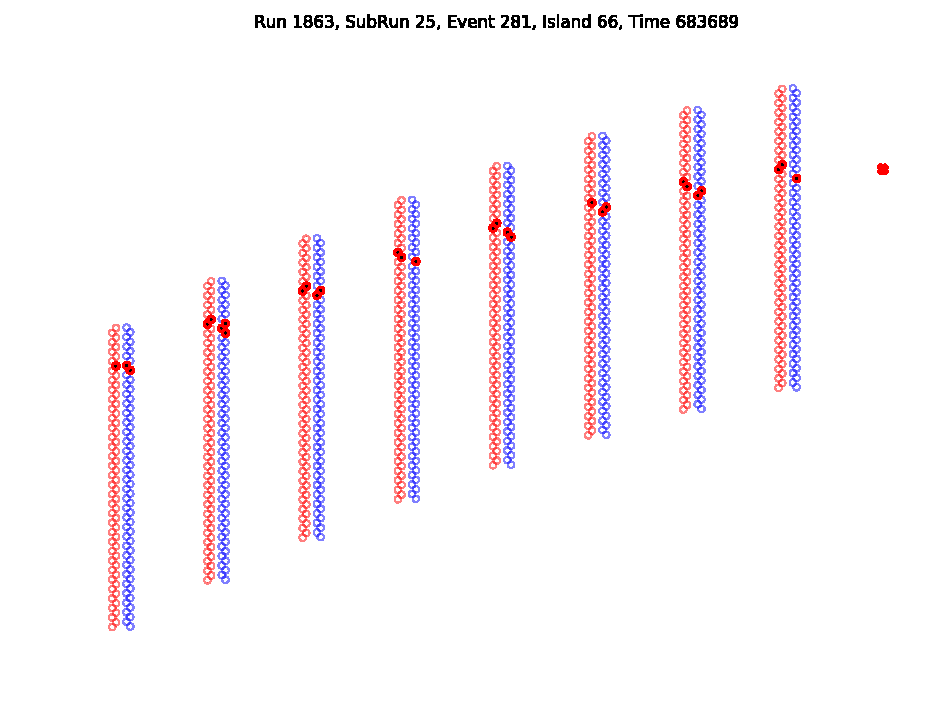
\includegraphics[width=0.9\textwidth]{TrackAndCaloHit}
    \caption[TrackAndCaloHit]{clean up and possibly replace}    
    \label{fig:TrackAndCaloHit}
\end{figure}

\begin{figure}[]
	\centering
	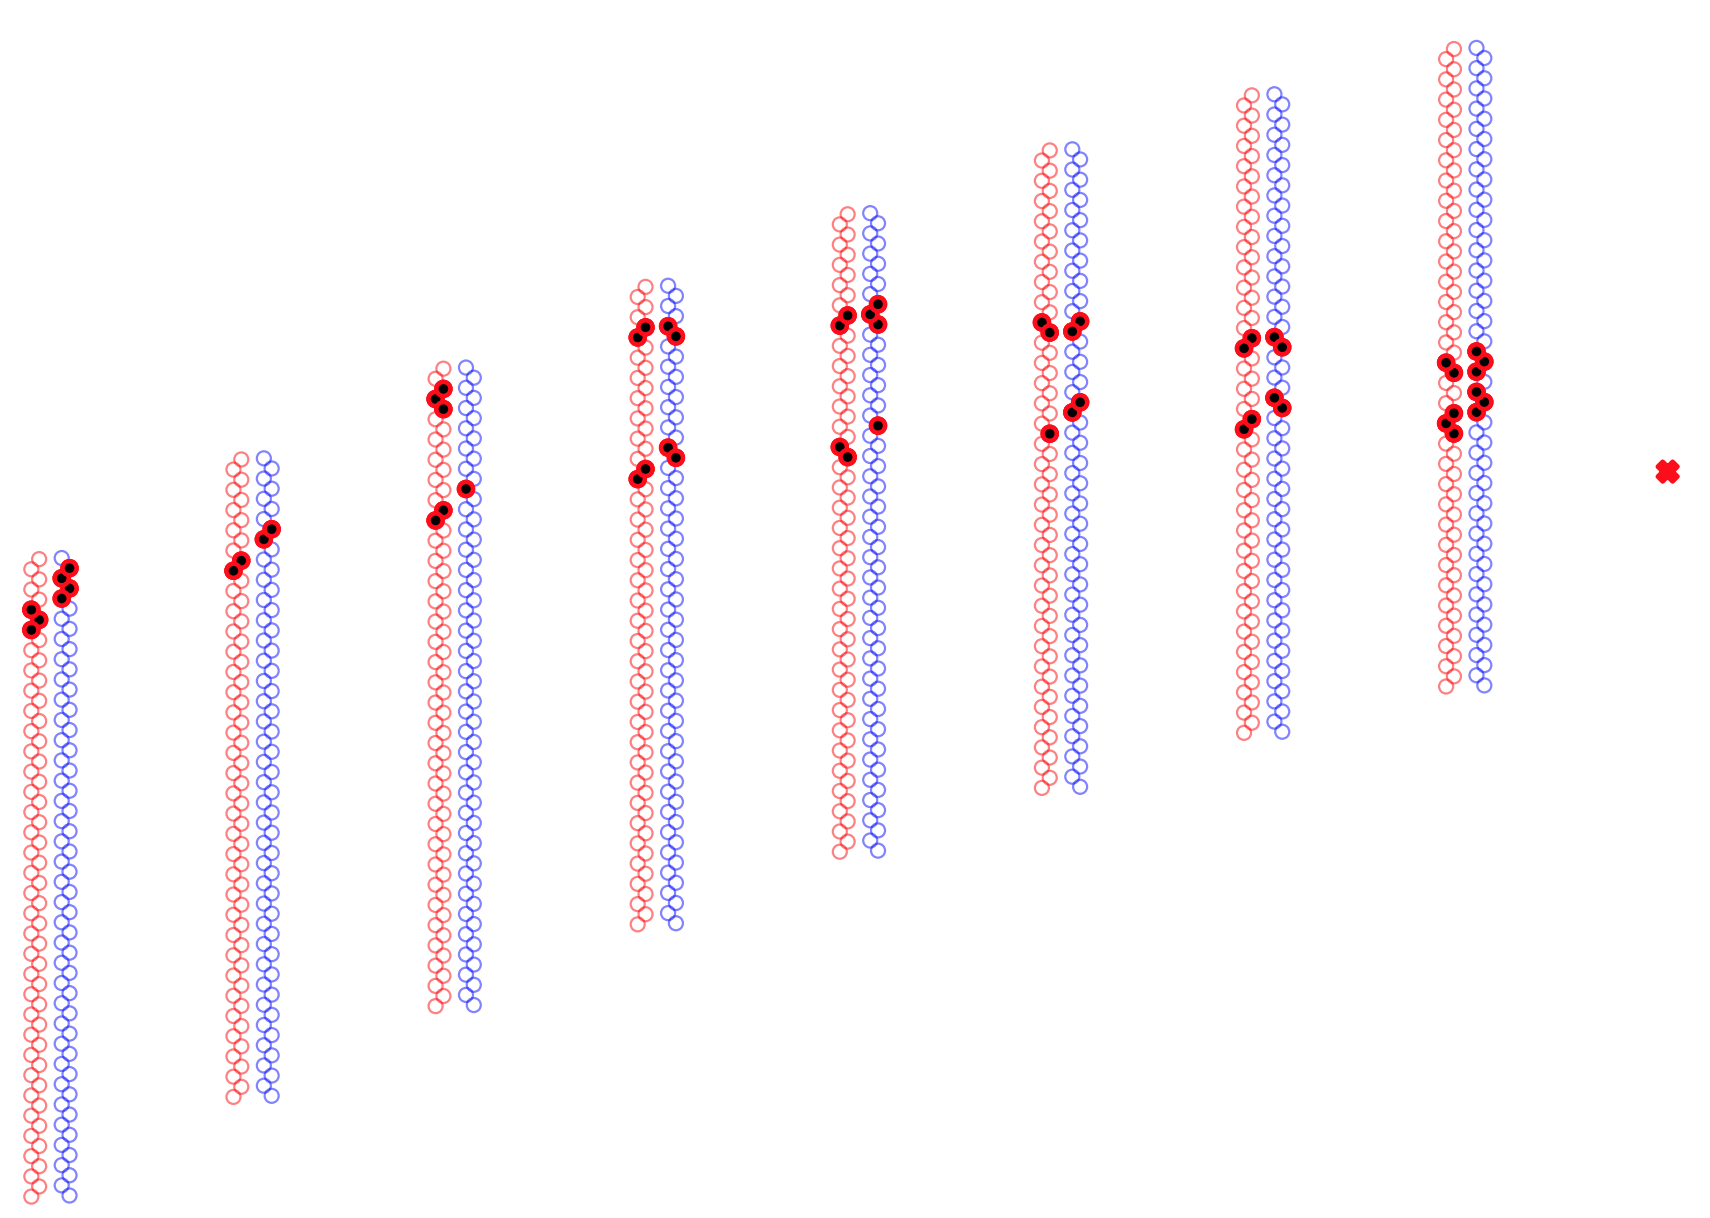
\includegraphics[width=0.9\textwidth]{pileupEvent}
    \caption[pileupEvent]{clean up and possibly replace}    
    \label{fig:pileupEvent}
\end{figure}




\section{Track Fitting}
\label{sec:TrackFitting}

The Geane fitting routines originated in Fortran with the EMC collaboration, and was used in the precursor E821 experiment as well as the PANDA experiment with some success \cite{geanemanual}, \cite{Lavezzi}. (I'm not actually aware of a useful reference for it's use in E821, and there are some other instances of its use as well in other experiments. In E821 there was a single tracking chamber which was never put to full use.) The core error propagation routines were at some point added to Geant4 under the error\_propagation directory which is included in all default installs. The tracking code strengths lie with its direct implementation and access to the Geant4 geometry and field, and its ability to handle the field inhomogeneties. The Geane fitting algorithm code which makes use of the Geant4 error propagation routines follows the structure of \cite{geanemanual} and is detailed in the \hyperref[sec:Formalism]{Formalism} section in this paper. It is a relatively straight forward least squares global \chisq minimization algorithm. 


Because of the proximity of the trackers to the muon beam, they will lie within a region of varying magnetic field. The radial field of the trackers rises from 0 Tesla at the outer ends to roughly .3 Tesla at the inner top and bottom ends, and the vertical field drops approximately 50\% from the storage dipole field of 1.451 Tesla. Shown in Figures \ref{fig:operaBy} and \ref{fig:operaBx} is the location of the tracker with respect to the horizontal and vertical fields respectively. These large field gradients over the tracking detector region and the long extrapolation distance back to the muon decay point are special to Muon \gmtwo. This is one of the main motivations for using the Geane fitting algorithm and routines, which has direct access to the field.

\begin{figure}[]
	\centering
	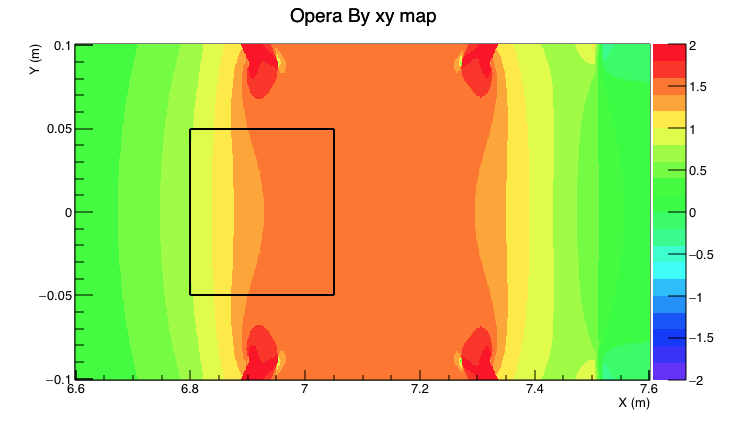
\includegraphics[width=0.9\textwidth]{operaBy}
    \caption[Vertical magnetic field from Opera2D]{Shown is the vertical field of the \gmtwo magnet in and around the storage region as calculated in Opera 2D. The center of the storage region lies at 7.112 m along the x axis. The black box shows the rough location of the tracker with respect to the field (size exaggerated slightly). It can be seen that there is a large inhomogeneity within the tracker space, goring from left to right.}
    \label{fig:operaBy}
\end{figure}

\begin{figure}[]
	\centering
	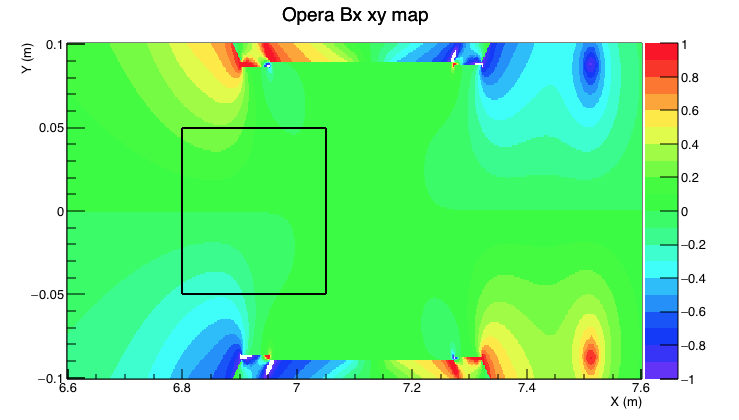
\includegraphics[width=0.9\textwidth]{operaBx}
    \caption[Horizontal magnetic field from Opera2D]{Shown is the radial field of the \gmtwo magnet in and around the storage region as calculated in Opera 2D. The center of the storage region lies at 7.112 m along the x axis. The black box shows the rough location of the tracker with respect to the field (size exaggerated slightly). It can be seen that there is a large homogeneity at the inner upper and lower ends compared to the right center. The shape of the pole pieces and tips can readily be seen.}
    \label{fig:operaBx}
\end{figure}



% \subsection{Track Fitting Formalism}
% \label{sec:TrackFittingFormalism}

    I recommend reading \cite{geanemanual}, Chapter 4 of \cite{Lavezzi}, and \cite{trajfit} in order to best understand the fitting algorithm. However, due to the at times confusing notation, ommitted equations or concepts, and differences between papers, I have attempted to summarize here the different sources and present the material in a more understandable and readable format. The implementation of the fitting algorithm into the code follows this section.

    One can define a $\chi^{2}$ for a track in the usual way by dividing the residuals of measured and predicted track parameters by their errors:
        \begin{align} \label{eq:chi2}
            \chi^2 = (\vec{p}-\vec{x})^{T} (\sigma^{-1}) (\vec{p}-\vec{x}),
        \end{align}
    where $\vec{p}$ are predicted track parameters from a fit to the measured track parameters $\vec{x}$, and $\sigma$ is a covariance matrix of errors on the fitted parameters. The Geant4 error propagation routines can be used to determine these predicted parameters and error matrices by propagating track parameters from some initial guesses. By minimizing this $\chi^{2}$ with respect to the track parameters one can then fit and improve the track. The Geant4 error propagation routines propagate particles along their average trajectories neglecting the effects of discrete processes, using a helix equation along small enough steps where the change in the magnetic field is small. The predicted parameters are then a function of path length: 
        \begin{align} \label{eq:pp}
            p_{l} = F_{l,l_{0}}(p_{0}),
        \end{align}
    where the path length can be defined how one wishes. In our system we have tracker planes defined at X positions, and limit path lengths to reach those planes. (From here on the dependence on path length or X position will be neglected, in favor of using plane indices.) In tandem, error matrices describing the expected distribution in true parameters about those predicted parameters due to said discrete process are also calculated:
        \begin{align} \label{eq:sigma}
            \sigma^{ij} = <p^{i}p^{j}> - <p^{i}> \cdot <p^{j}>,
        \end{align} 
    where i and j are track parameter indices. These parameter vectors are 5x1 objects defined in some track representation, as described in the \hyperref[sec:Coord]{Coordinate Systems} section. The propagation of these parameters and error matrices are done using transport matrices, which express the infinitesimal changes in parameters at some plane (or path length) with respect to the parameters at some previous plane (or previous path length):
        \begin{align} \label{eq:transport}
            \delta p_{N} &= T_{N,N-1} \delta p_{N-1}, \\
            \sigma_{N} &= T_{N,N-1} \sigma_{N-1} T_{N,N-1}^{T}.
        \end{align}
    Said transport and error matrices are 5x5 objects since the parameter vectors are 5x1 objects as described above. The calculation of these transport matrices, as well as details on the functional form of \ref{eq:pp} are shown in \cite{jacob}.

    With parameters defined on such planes, one can define the $\chi^{2}$ as: 
        \begin{align} \label{eq:chi2sum}
            \chi^2 = \sum_{i=1}^{N} [(p_{i}(p)-x_{i})^{T} (\sigma_{i}^{-1}) (p_{i}(p)-x_{i})],
        \end{align}
    where $p_{i}$ are the average predicted parameters from some general starting parameters $p$. At first order one can solely include the measurement errors on parameters, which fill in the diagonals of $\sigma_{i}$, if random processes can be neglected. Unmeasured parameters should have measurement errors of infinity (or some large value) along the diagonals in the code, which account for the fact that residuals for unmeasured parameters do not exist. When the error matrix is inverted all rows and columns of the matrix with these large numbers will fall to 0 in the $\chi^{2}$. 

    In order to get the best fit track, the $\chi^{2}$ should be minimized with respect to the initial track parameters p, and evaluated at some chosen or fitted parameters:
        \begin{align} \label{eq:minimize}
            \frac{\partial \chi^{2}}{\partial p}|_{p=p'_{0}} = 0,
        \end{align}
    resulting in
        \begin{equation}
        \begin{aligned}
            0 = \sum_{i=1}^{N}[ (\frac{\partial p_{i}(p)}{\partial p}|_{p=p'_{0}})^{T} (\sigma_{i}^{-1}) (p_{i}(p'_{0})-x_{i}) \\ 
            + (p_{i}(p'_{0})-x_{i})^{T} \frac{\partial(\sigma_{i}^{-1})}{\partial p}|_{p=p'_{0}} (p_{i}(p'_{0})-x_{i}) \\ 
            +  (p_{i}(p'_{0})-x_{i})^{T} (\sigma_{i}^{-1}) (\frac{\partial p_{i}(p)}{\partial p}|_{p=p'_{0}})]
        \end{aligned}
        \end{equation}
    where the 1st and 3rd terms are identical, and the 2nd term is small if one assumes that the error matrix doesn't change much with respect to the starting parameters. (Fair since most of the error comes from measurement, and as long as the initial guess is decent enough such that the path length through material doesn't change appreciably from one iteration to the next.) This simplifies to: 
        \begin{align} \label{eq:solve}
            \sum_{i=1}^{N} T^{T}_{i0} (\sigma_{i}^{-1}) (p_{i}(p'_{0})-x_{i}) = 0,
        \end{align}
    which is just the top term with 
        \begin{align} \label{eq:transport2}
             T_{i0} = \frac{\partial p_{i}(p)}{\partial p}.
        \end{align}
    To solve this make the substitution 
        \begin{align} \label{eq:psub}
            p_{i}(p'_{0}) = p_{i}(p_{0}) + \frac{\partial p_{i}(p_{0})}{\partial p} \Delta p_{0} = p_{i}(p_{0}) + T_{i0} \Delta p_{0},
        \end{align}
    where $p'_{0}$ are the improved starting parameters for the next iteration calculated from the previous starting parameters $p_{0}$, and $\Delta p_{0}$ are the changes in the starting parameters to improve the track. This equation can be plugged into the above if one makes the assumption that $T_{i0}$ does not change much from one iteration the next, which follows from the inherent nature of making small adjustments to the track in order to improve it.

    After simplifying one arrives at 
        \begin{align} \label{eq:deltap}
            \Delta p_{0} = \sigma_{p_{0}} \sum_{i=1}^{N} T^{T}_{i0}(\sigma_{i}^{-1})(x_{i} - p_{i}(p_{0})),
        \end{align}
    where
        \begin{align} \label{eq:cov}
            \sigma_{p_{0}} = [\sum_{i=1}^{N} T^{T}_{i0} (\sigma_{i}^{-1}) T_{i0} ]^{-1},
        \end{align}
    is the 5x5 covariance matrix of fitted parameters on the starting plane, whose diagonals describe the errors in the 5 track parameters on that plane and in the region close to it. (The fit does not directly return fit errors for track parameters on other planes.) $\Delta p_{0}$ along with $\chi^2$ is exactly what we want to determine since that is what allows us to fit and improve the track from iteration to iteration.

    However, since random processes should not be neglected for optimal tracking results, it makes more sense to return to the original $\chi^2$ in equation \ref{eq:chi2}, only now the included matrix and vector objects are combined into one large linear algebra equation. Instead of a sum over N 5x1 objects multiplying 5x5 error matrices, the vectors are combined into a single 5Nx1 vector multiplying a single 5Nx5N matrix. The 5x5 diagonal blocks of this large error matrix should now include the effects due to material processes as calculated in Geant from equation \ref{eq:sigma} as well as the measurement errors. 

    Because now parameters at one plane are no longer independent of the parameters at other planes, due to correlations from these random processes, it's necessary to add off-diagonal elements into the large error matrix. These 5x5 blocks come from 
        \begin{align} \label{eq:corr}
            \sigma_{MN} = T_{MN} \sigma_{N}, 
        \end{align}
    for the top diagonals, and the transpose for the bottom diagaonals, where M and N are two separate planes within the detector. ($\sigma_{N}$ is the error matrix on plane N calculated from the starting plane.) This follows from equation \ref{eq:sigma} evaluated at plane M with respect to a path length from plane N, and not plane 0, which is equivalent to \ref{eq:corr}. 

    You can then minimize the $\chi^{2}$ in the same way, only again with the matrix objects being aggregates of the per plane objects:
        \begin{align} \label{eq:deltafull}
            \Delta \vec{p}_{0} = \sigma_{p_{0}} \tau^{T}\sigma^{-1}(\vec{x}-\vec{p}),
        \end{align}
        %
        \begin{align} \label{eq:covfull}
            \sigma_{p_{0}} = [\tau^{T} \sigma^{-1} \tau ]^{-1},
        \end{align}
    where $\tau$ is the combined transport matrices from the individual 5x5 matrices, a 5Nx5 object.

    The unmeasured parameter errors of infinity still come into play in the final calculation in the same was as before. Because however these matrix objects are very large, and the tracking must have a certain amount of speed in order to keep up with data, it is useful to reduce the size of these matrices. (It also makes things easier programming wise. Note that there are other some other ways to speed things up, specifically the banded inversion method as described in reference \cite{trajfit}. This method was not used in favor of getting the code working in the simpler form in the first place, but it is a possiblity in the future to use this technique to speed things up even more.) It suffices to simply remove all rows and columns where said infinity values exist in the error matrix. This is mathematically equivalent to inverting the error matrix with the infinities included, which make all rows and columns where they exist go to zero. The associated unmeasured parameter rows in the residual vector and transport matrices must similarly be removed. This results in an Nx1 residual vector, NxN error matrix, 5xN combined transport matrix transpose, which multiply against the 5x5 covariance matrix out front to still result in a 5x1 fix to the starting parameters, and a scalar $\chi^2$ value. (Note that these element removals should be done just before the final calculation, and not higher up in the algrebra, otherwise plane correlations are not properly calculated.)

    By calculating the last two equations one can fit the track, acquire a $\chi^{2}$ describing the degree of the fit, determine how the track parameters can be improved at the starting point, and calculate errors on those starting parameters. This algorithm can be iterated a number of times to get a best fit track until successive iterations produce no improvement, where usually 3 or 4 iterations is enough. Note that there is remarkable robustness with respect to the initial starting parameters in fitting the track. Of course if the initial starting paramaters are too poor, then the fit will not converge. All of these calculations are completed within the \hyperref[sec:GeaneFitter]{GeaneFitter.cc} file within the framework.




-don't forget about angular correction in appendix of fitting documentation - might want to put that in the appendix of my thesis




\section{Track Extrapolation}
\label{sec:TrackExtrapolation}





\begin{figure}[]
	\centering
	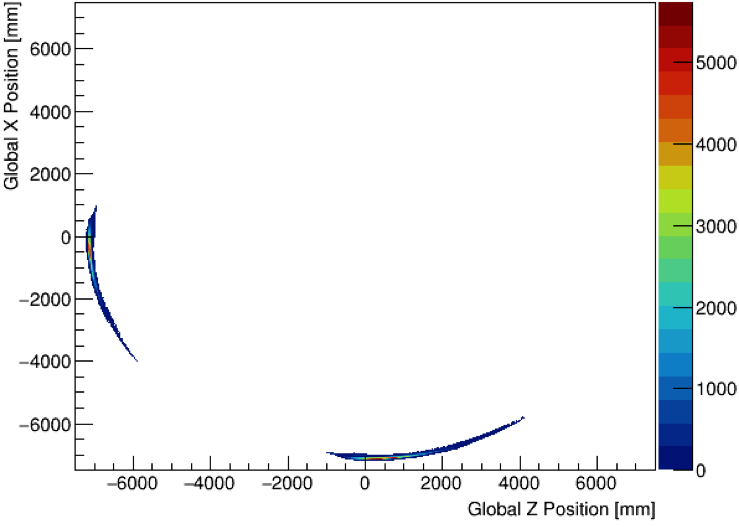
\includegraphics[width=0.9\textwidth]{BirdsEyeExtrapPreliminary}
    \caption[Birds Eye View of Extrapolation]{preliminary replace at some point}    
    \label{fig:BirdsEyeExtrapPreliminary}
\end{figure}

\begin{figure}[]
	\centering
	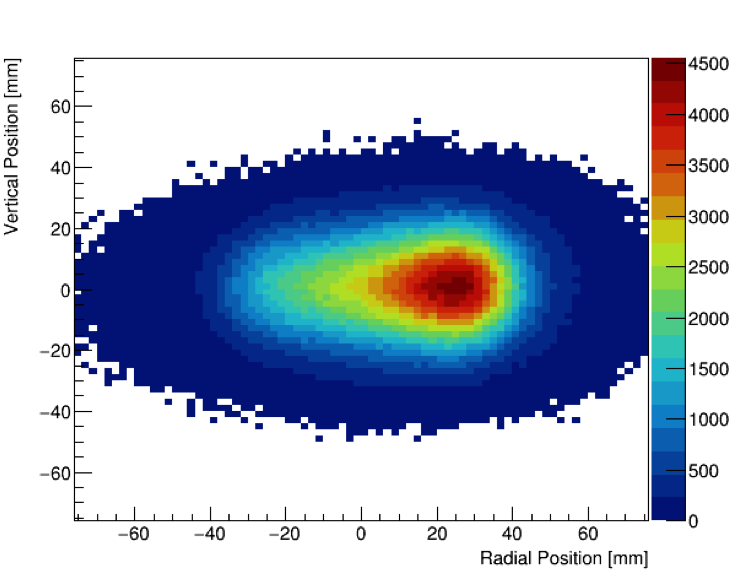
\includegraphics[width=0.9\textwidth]{BeamSpotPreliminary}
    \caption[Beam spot extrapolation]{preliminary replace at some point}    
    \label{fig:BeamSpotPreliminary}
\end{figure}


